\documentclass[a4paper,11pt]{book}
\usepackage{import}
\usepackage{preamb}

\makeindex

\begin{document}

\small
\begin{multicols}{3}

%\maketitle

\thispagestyle{empty}
\scriptsize
\newpage


\begin{subbox}{subbox}{}
\centering
\Large{\textbf{Network Science   \\ Cheatsheet}}
\end{subbox}

\begin{multibox}{2}
\begin{subbox}{subbox}{}
\centering

\includegraphics[width=0.8\textwidth]{pics/logo.png}
\end{subbox}
\begin{subbox}{subbox}{}
\centering
Made by \\
\large{
Remy Cazabet
}
\end{subbox}
\end{multibox}
% \section{Blocks and Community structure}


\begin{subbox}{subbox}{}
\centering
\Large{\textbf{Scale-Free Networks}}
\end{subbox}

\begin{textbox}{Scale-Free: Definition}

A network is said to be \textbf{Scale-Free} when its degree distribution follows a Power-Law distribution, or can be approximated by a Power-Law distribution. 

\end{textbox}

\begin{textbox}{Power-Law (PL)- Approximate Distribution}

A \textbf{Power-Law distribution} is defined as follows:
\[
P(k) \sim k^{-\alpha} = \frac{1}{k^\alpha}
\]

$\alpha$ is called the \textit{exponent} of the distribution.

Intuitively, the more $\alpha$ is large, the more large values are rare. For instance, with $\alpha=0$, it corresponds to a uniform distribution (any degree is equivalently probable). With $\alpha=1$, the probability of a node taken at random to have degree $k$ is $\sim \frac{1}{k}$. Usually, a distribution is considered scale free when $2\leq \alpha\leq 3$, as we will see.

\end{textbox}


\begin{textbox}{PL - Boundaries}

In most settings, the Power-Law degree distribution exists only for a certain range of degrees. 

This makes sense in real networks: few people have 0 or 1 social contacts, for instance, few websites have no incoming nor outgoing hypertext links, or we wouldn't even be aware of them. Thus there is a \textbf{lower bound} $k_{min}$ from which the distribution exists. 

Similarly, real networks represent entities of the real world, which are in finite numbers, therefore the number of elements itself is a limit. But in many situations, even lower thresholds exist: Social networks often impose a limit to the number of connections to avoid spammers, time and space also typically impose limits to what is possible or not in a network. An \textbf{upper bound} $k_{max}$ can be used to limit the distribution. 

\end{textbox}


\begin{textbox}{Power-Law - Exact Distribution}

For a distribution to be properly defined, the sum of all probability must be equal to one, we therefore add a normalization constant $C$ to ensure this property.
\[
\int P(k)=1= \int Ck^{-\alpha}=C\int k^{-\alpha}
\]
From which we can define $C$:
\[
C = \frac{1}{\int_{k_{\min}}^{\infty}k^{-\alpha} dk}=(\alpha-1)k_{\min}^{\alpha-1}
\]
And finally, the exact definition of the Power-Law degree distribution with lower bound:
\[
P(k) = (\alpha-1)k_{\min}^{\alpha-1}k^{-\alpha} \\
P(k) = \frac{\alpha-1}{k_{\min}}\left(\frac{k}{k_{\min}}\right)^{-\alpha}
\]

\end{textbox}






\begin{textbox}{Power-Law - Plotting}

A famous property of the Power-Law distribution is that it looks like a line when plotted in a log-log plot, i.e., a plot in which the x-axis (degrees) and the y-axis (frequency of degrees) are represented using a logarithmic scale.
\begin{center}
Power-Law distributions in linear scale for degrees [1-10] \\
(100 000 samples)

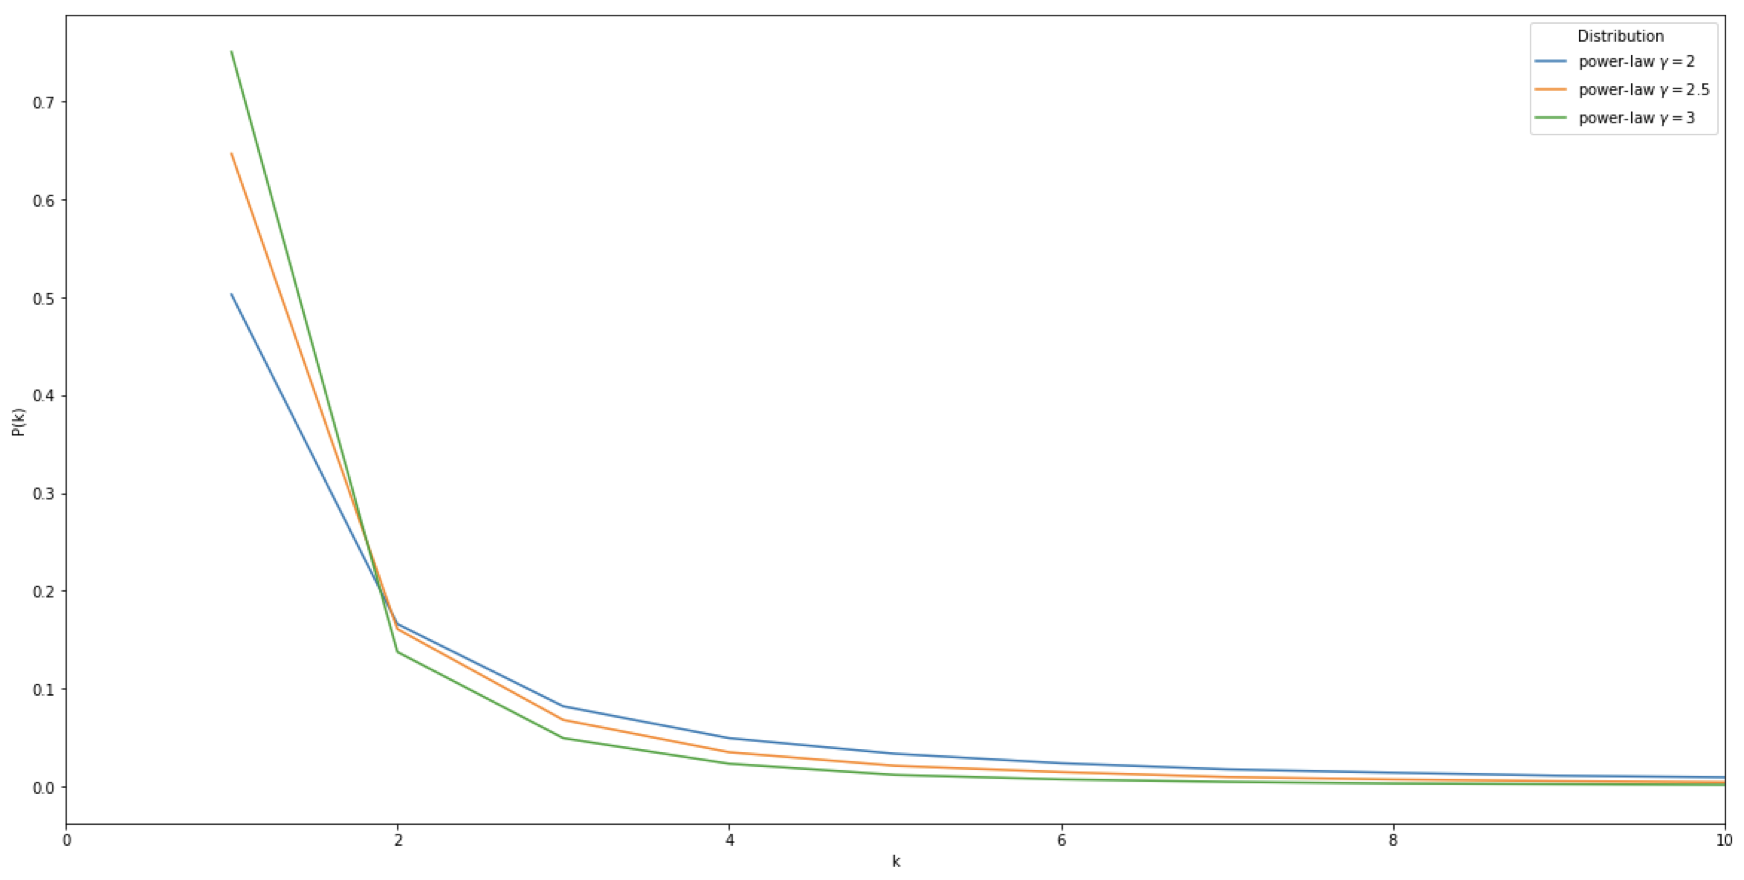
\includegraphics[width=0.5\textwidth]{pics/SF1.png}

Power-Law distributions in linear scale for degrees [1-100000] \\
(100 000 samples). The distribution is so heterogeneous that is is not readable.

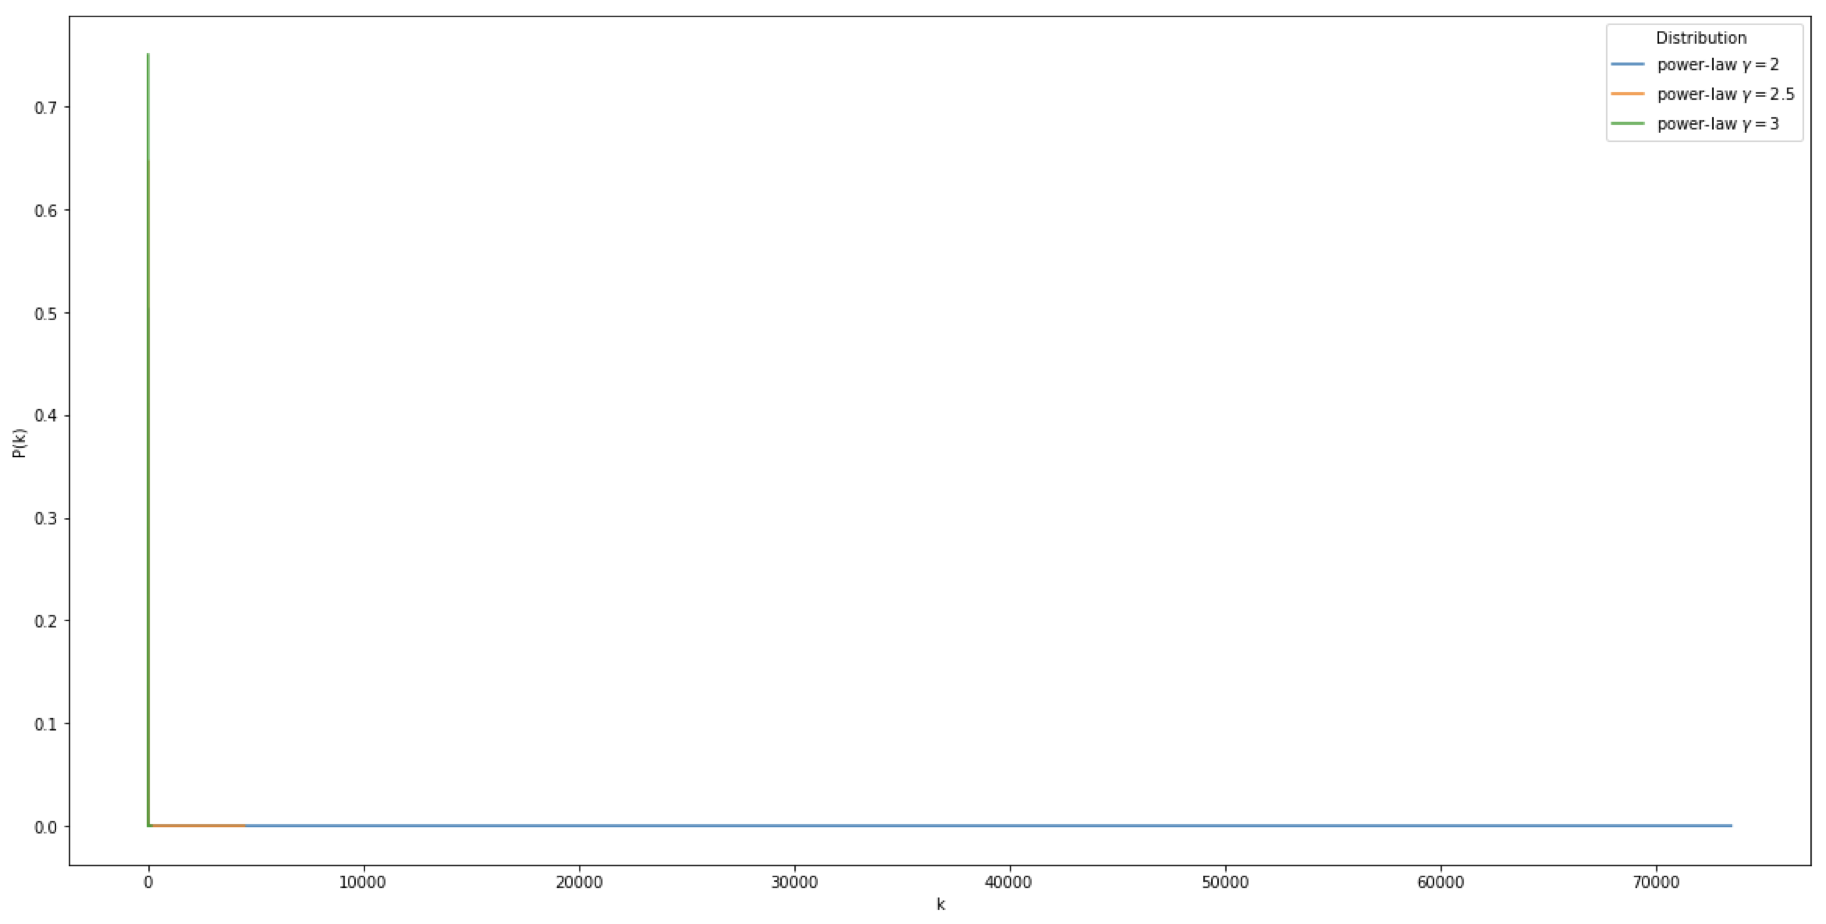
\includegraphics[width=0.5\textwidth]{pics/SF2.png}

Power-Law distributions in log-log scale for degrees [1-100000] \\
(100 000 samples).

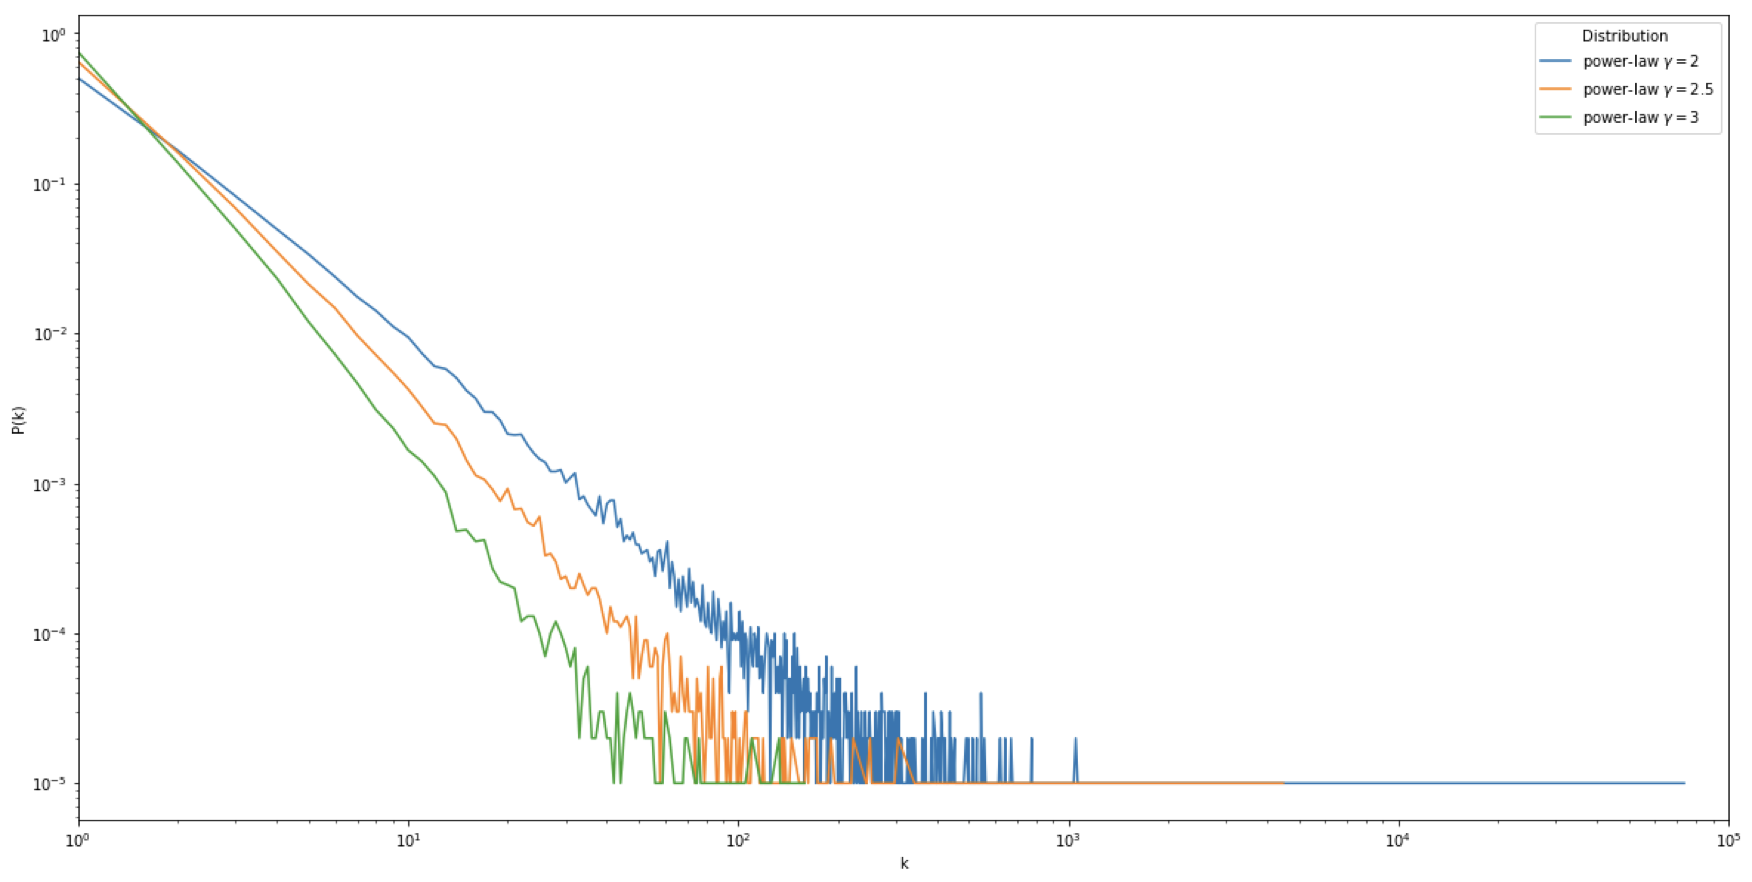
\includegraphics[width=0.5\textwidth]{pics/SF3.png}
\end{center}

\end{textbox}








\begin{textbox}{Power-Law - Long tail}

Compared with other well-known distributions such as Poisson or exponential distribution, a key difference is what is called the \textbf{long-tail} property: very large values are rare, but possible. We can observe this long tail by comparing with other distributions on log-log plots.

\begin{center}
Comparing power-law with Poisson distributions
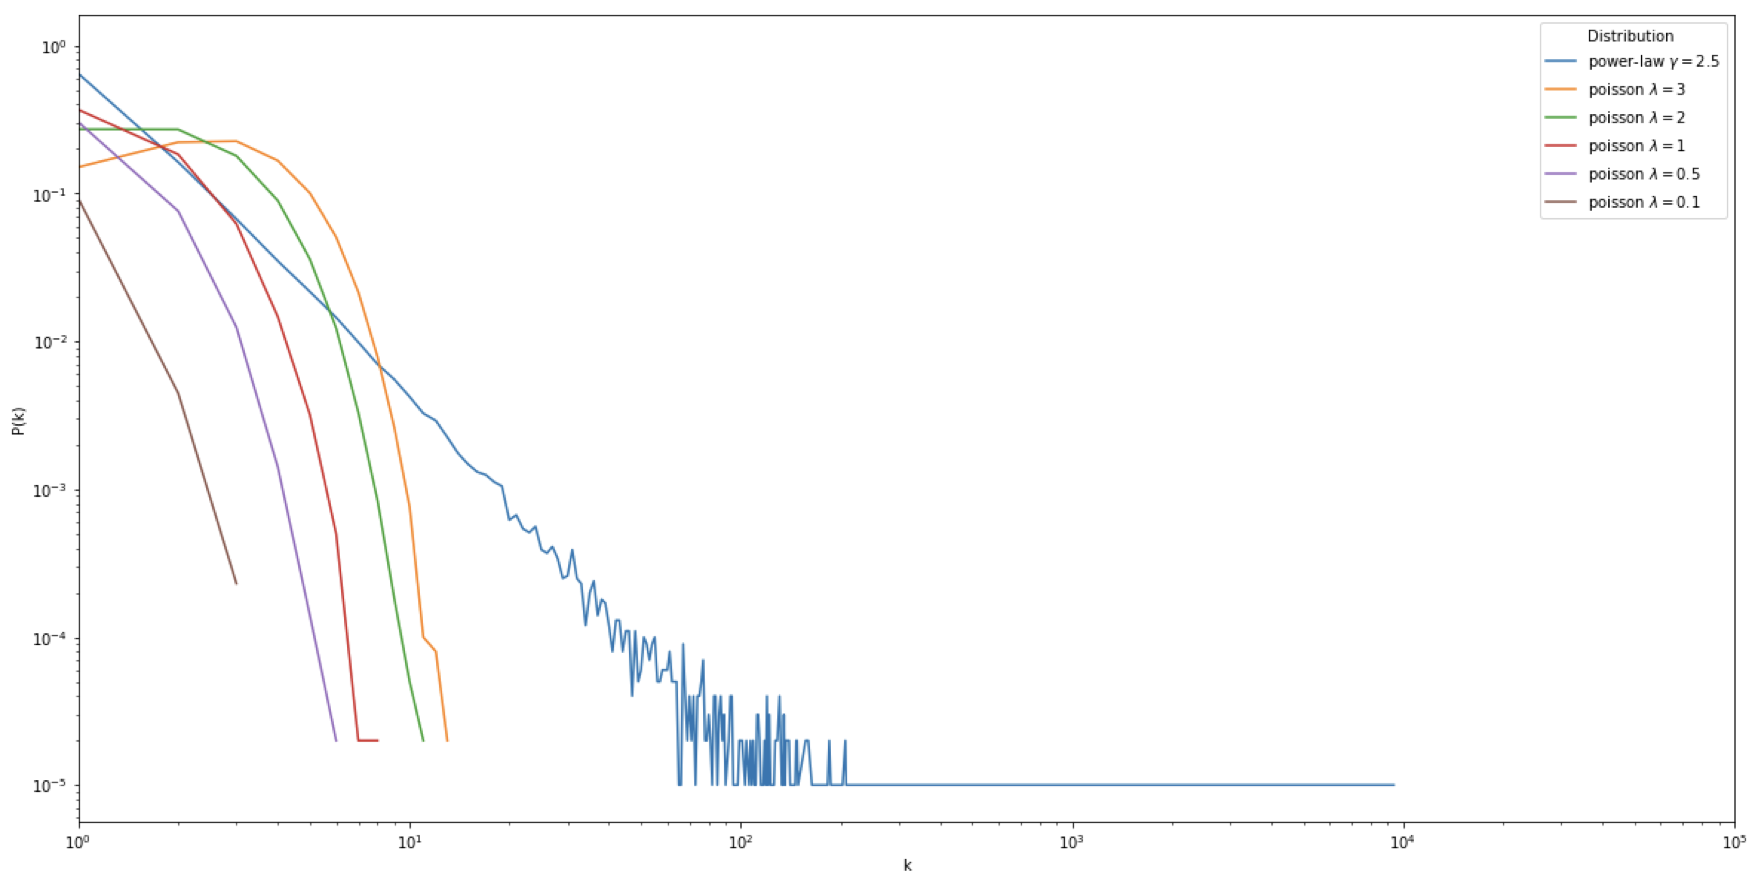
\includegraphics[width=0.8\textwidth]{pics/SF-poisson.png}

Comparing power-law with Exponential distributions


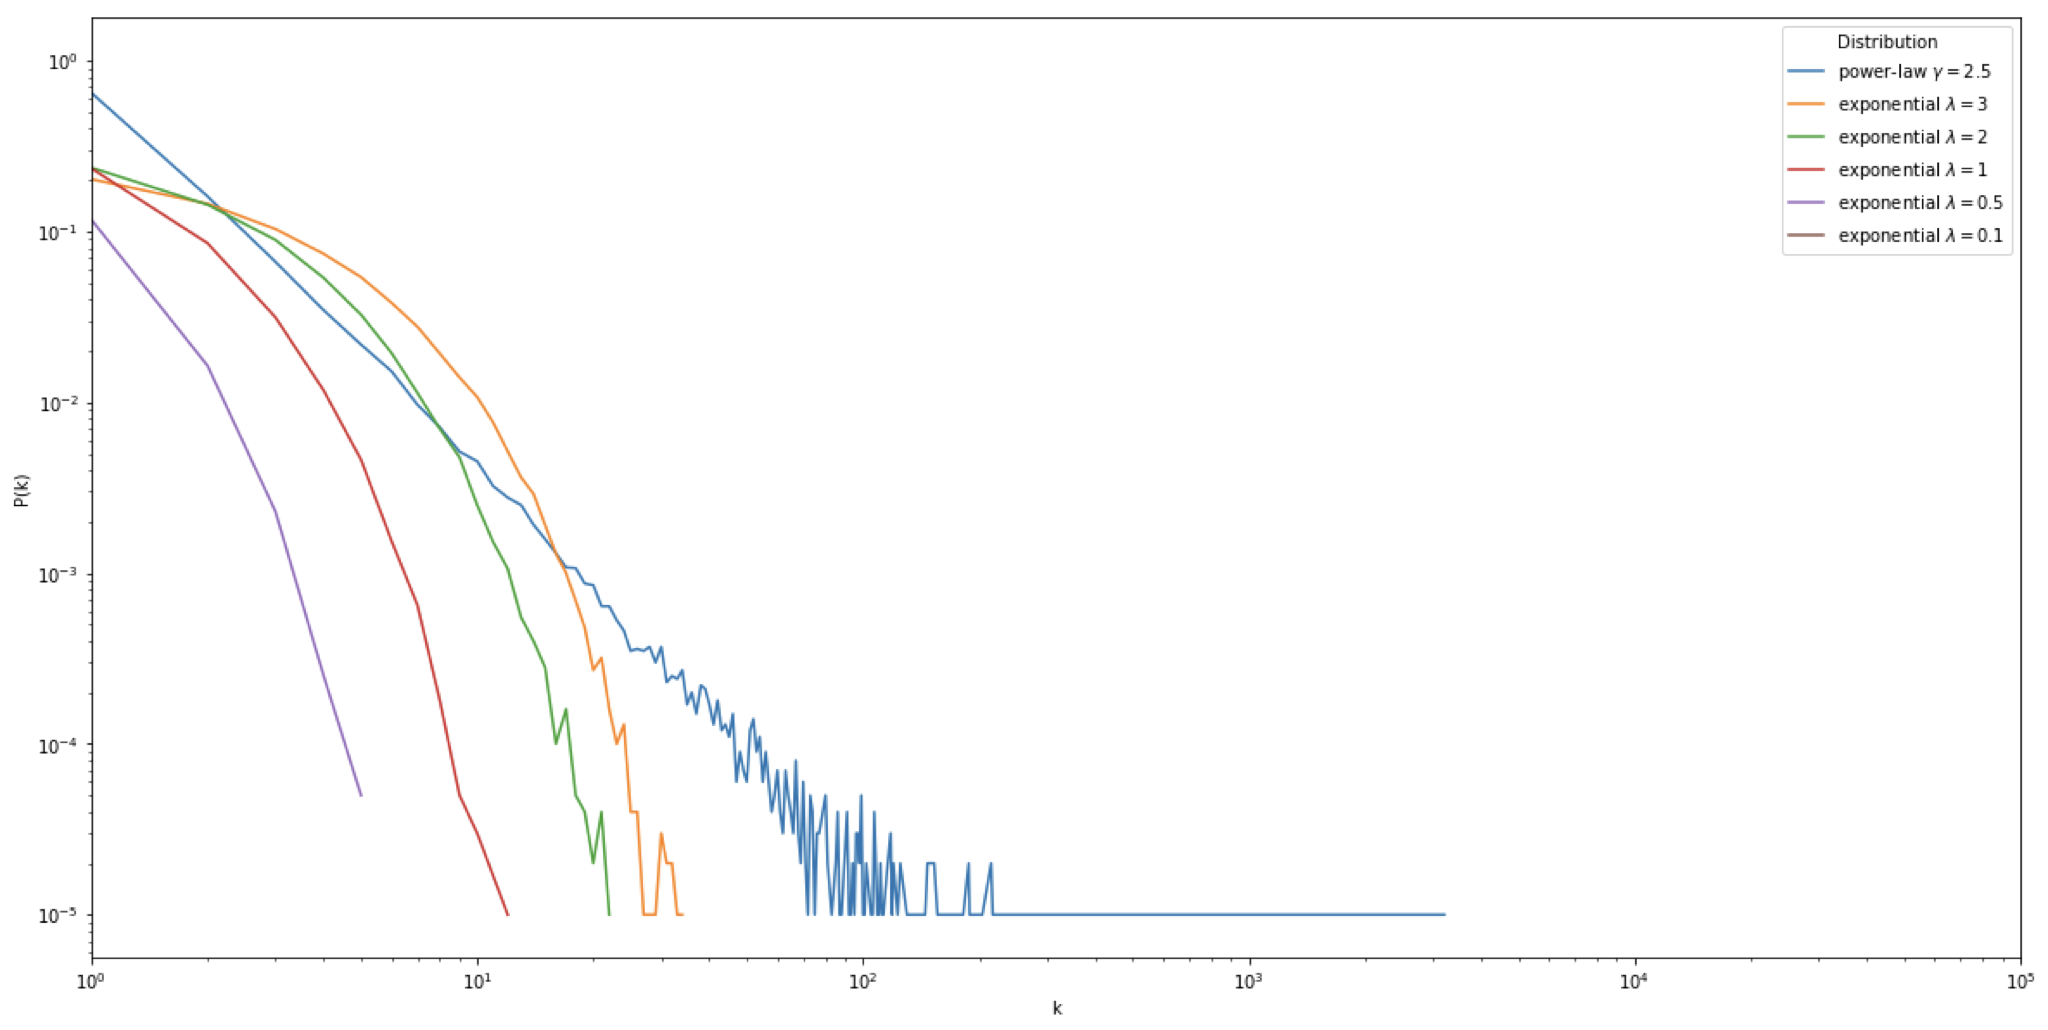
\includegraphics[width=0.8\textwidth]{pics/SF-exponential.png}

\end{center}

\end{textbox}




\begin{textbox}{SF networks - universality}

Scale-Free networks are widely studied because they are considered to be very frequent in the real world. Some important papers discovered the existence of Power-Law degree distribution in a variety of large real networks, notably:
\begin{enumerate}
    \item The World Wide Web (webpages) (\cite{barabasi1999emergence})
    \item The internet (physical network) (\cite{faloutsos1999power})
    \item Airline connections (\cite{guimera2004modeling})
    \item Scientific collaborations (\cite{newman2001structure})
    \item Romantic interactions (\cite{liljeros2001web})
\end{enumerate}

It must be noted, however, that many real world networks \textbf{are not scale-free}. A typical counter-example is a road-network, in which nodes correspond to intersection and edges to roads: for practical reasons, intersections with large degrees do not make sense.

\end{textbox}






\begin{textbox}{Why is it called \textit{scale free}}

Because they have no (typical) scale! 

It is defined in opposition to Poisson and other Bell-Shaped distributions, which are \textbf{centered around their average value}. Let's take a typical example: The height of humans follow a Bell-shaped distribution: the average height is 1.65m, and most humans are quite close to this value, there is a \textbf{typical scale} of human height. On the contrary, human wealth distribution follows approximately a power-law \footnote{ \url{https://en.wikipedia.org/wiki/Distribution_of_wealth}}: a few humans are extremely wealthy (Billions of \$), while more than half the world population posses less than 10 000\$. As a consequence, the average human wealth (70 000\$) is not at all representative of human wealth.


\end{textbox}


\begin{textbox}{Central moments}
The first two central moments of a distribution are the mean $\langle k^1 \rangle $ and the variance $\langle k^2 \rangle $. They are defined as 
\[
\langle k^m \rangle = \int_{k_{\min}}^{\infty}k^mp(k)dk=(\alpha-1)k^{\alpha-1}_{\min}\int_{k_{\min}}^{\infty}k^{-\alpha+m}dk
\]
From this, we can conclude that \textbf{central moments are defined only if $\alpha>m+1$}, otherwise they diverge towards infinity, they are not properly defined.

Thus:
\begin{enumerate}
    \item $\langle k^2 \rangle = \frac{\alpha-1}{\alpha-2}k_{\min}$, \textbf{if and only if $\alpha\geq 2$}
    \item $\langle k^3 \rangle = \frac{\alpha-1}{\alpha-3}k^2_{\min}$, \textbf{if and only if $\alpha\geq 3$}
\end{enumerate}



\end{textbox}



\begin{textbox}{Divergence in practice}
In practice, one can always compute the mean and variance of a provided, observed degree distribution. So what does it mean that they \textit{diverge}?

The problem arises when we are not certain to observe the whole network. Usually, a large sample of a population has the same mean and variation than the whole population, and the largest the sample, the more precise the value.

But in a power law, moments are \textbf{dominated} by the largest values in the long tail: some rare values are \textit{so large} that they shift the moments. So the more data we observe, the higher the moments.
\end{textbox}

\begin{textbox}{Divergence: consequences}
The consequence of diverging moments is that \textbf{if the distribution follows a power law}, then if the exponent is below 2, you should now rely on the mean degree or the variance. If the exponent is between 2 and 3, you can (relatively) rely on the mean, but not on the variance. Be careful though, even if $\alpha>2$, the mean converges slowly, i.e., you need a very large sample for your mean to be close to the real value.
\end{textbox}

\begin{textbox}{Fitting power laws}
When confronted with a power law degree distribution, we might want to \textbf{fit} the distribution, i.e., to \textbf{find the exponent} of the distribution. A naive and simple way to do it is to plot the distribution on a log-log plot and to find the slope of the line, either graphically or through least-square regression on the log-transformed values of degrees and frequencies. 

This however suffers from a strong bias: values in the tail are based on a few samples, and introduce noise.

The most appropriate method is to use Maximum Likelihood Estimation (MLE\footnote{https://towardsdatascience.com/a-gentle-introduction-to-maximum-likelihood-estimation-9fbff27ea12f}), taking into account min and max-boundaries, as described in \footcite{goldstein2004problems}
\end{textbox}

\begin{textbox}{Exponent limits}
In real networks, we consider that we should have $\alpha\geq2$, because a lower exponent would mean that the distribution is so skewed that we expect to find nodes with a degree larger than the size of the network.

Furthermore, if the exponent is too large, large degree nodes becomes so rare, that the network would need to be enormous to observe such a node. For instance, with $\alpha=5$, we need to observe $N=10^{12}$ nodes to expect to observe a single node of size 1000.
\end{textbox}

\begin{textbox}{Exponent and shortest-paths}
Random networks with Poisson degree distribution already have a \textit{short average distance}. However, it is possible to define classes of networks with even smaller average distance based on the exponent $\alpha$:
\begin{itemize}
    \item $\alpha=2$: The biggest hub degree is of order $\mathcal{O}(N)$, thus most nodes are at distance 2. The average path length can be considered a small constant, independent of $N$
    \item $2<\alpha<3$: \textbf{Ultra Small World}: $\langle \ell \rangle = \frac{\log \log N}{\log(\alpha-1)}$
    \item $\alpha=3$: $\langle \ell \rangle = \frac{ \log N}{\log \log N}$
    \item $\alpha>3$: $\langle \ell \rangle = \log N$, the network behaves approximately like an ER network.
\end{itemize}
\end{textbox}

\begin{textbox}{Scale-free network controversy}
There is an on-going debate in the network science community over the prevalence of scale-free networks. For some authors \footcite{barabasi2003scale}, most real networks follow to some extent a power-law degree distribution, while, for some others, scale-free networks are rare \footcite{broido2019scale}. The controversy has been studied\footcite{jacomy2020epistemic} and can be interpreted as differences between scientific approaches: one popular among (some) physicists (\textit{scale-freeness is the sign of a universal law}) and another one common among statisticians \textit{(scale-freeness is an empirical characterization)}.
\end{textbox}

\begin{textbox}{SF networks: what to do}
Is your network Scale-Free? The first question you might ask yourself is: \textit{why do you need to know?}. 
\begin{itemize}
    \item If the goal is to characterize a network, then plotting the degree distribution might be more useful than fitting a power-law exponent to it
 \item If the goal is to show that the distribution is broad, significantly different from a bell-shaped distribution, then plotting the distribution might be enough
 \item If the goal is to show that the distribution is \textit{approximately} a power-law, for instance because an algorithm complexity or a proof can be made for such cases, then fitting a line on a log-log plot and talking about \textit{power-law-ish} might be enough
 \item If on the contrary it is scientifically important to argue that the network is, without doubts, a scale-free networks, then you need to be fully aware of the controversy and to position your work relatively to it.  
\end{itemize}
\end{textbox}




 \AtNextBibliography{\footnotesize}


\printbibliography[heading=subbibliography]


\end{multicols}



\end{document}
